% vim: set tw=78 aw:
\documentclass{beamer}

\usepackage[utf8x]{inputenc}		% diacritice
\usepackage[romanian]{babel}
\usepackage{color}			% highlight
\usepackage{alltt}			% highlight
\mode<presentation>
{ \usetheme{Rochester} }		% TODO: settle this

% Titlul nu foloseşte Unicode pentru că e o problemă căreia nu i-am dat de
% cap.
\title[Proiect]{Nethack Clone}
\institute{ROSEdu}
\author{Andrei Buhaiu\\{\footnotesize andrewbwm@rosedu.org}}

\begin{document}

% Slide-urile cu mai multe părţi sunt marcate cu textul (cont.)
\setbeamertemplate{frametitle continuation}[from second]
% Arătăm numărul frame-ului
\setbeamertemplate{footline}[frame number]

\frame{\titlepage}


\begin{frame}{This is nethack}
\begin{figure}[h]
\centering
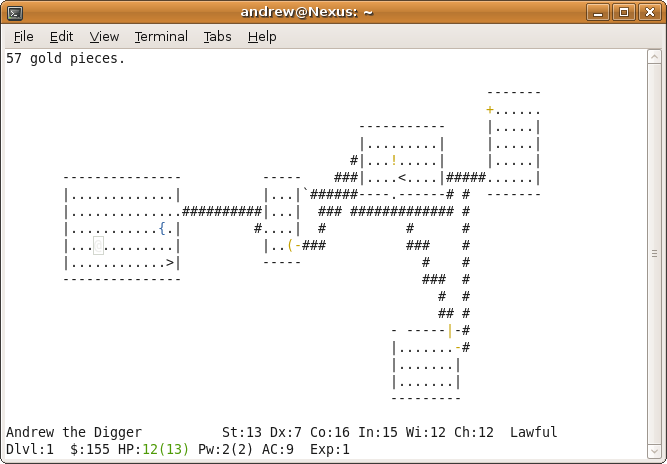
\includegraphics[scale = 0.3]{poza.png}
\newline
\centering
\text {O poză dintr-un joc de nethack}
\end{figure}
\end{frame}

\begin{frame}{Idea din spatele proiectului}
\begin{itemize}
\item Să se facă o clonă de nethack inițial mai simplă dar cu posibilități bune de dezvoltare ulterioară
\newline
\item Trebuie și bucăți de game design care pentru majoritatea sunt foarte plăcute, dar o durere de cap la implementare
\newline
\item Dacă se decide implementarea multiplayer-ului se vor folosi și sockets
\end{itemize}
\end{frame}

\begin{frame}{Tehnologii folosite}
\begin{itemize}
\item Python sau C
\newline
\item Cel mai probabil gtk pentru UI
\newline
\item Posibil și biblioteci de sockets dacă se vrea partea de multiplayer
\end{itemize}
\end{frame}

\begin{frame}{Motivație}
\begin{itemize}
\item Ceva simplu și distractiv
\newline
\item Cu posibilități mari de dezvoltare după
\newline
\item Ai cu ce să te joci după :P
\end{itemize}
\end{frame}

\end{document}
